%%%%%%%%%%%%%%%%%%%%%%%%%%%%%%%%%%%%%%%%%
% Simple Sectioned Essay Template
% LaTeX Template
%
% This template has been downloaded from:
% http://www.latextemplates.com
%
% Note:
% The \lipsum[#] commands throughout this template generate dummy text
% to fill the template out. These commands should all be removed when 
% writing essay content.
%
%%%%%%%%%%%%%%%%%%%%%%%%%%%%%%%%%%%%%%%%%

%----------------------------------------------------------------------------------------
%	PACKAGES AND OTHER DOCUMENT CONFIGURATIONS
%----------------------------------------------------------------------------------------

\documentclass[12pt]{article} % Default font size is 12pt, it can be changed here

\usepackage{subfigure}

\usepackage{geometry} % Required to change the page size to A4
\geometry{a4paper} % Set the page size to be A4 as opposed to the default US Letter

\usepackage{graphicx} % Required for including pictures

\usepackage{float} % Allows putting an [H] in \begin{figure} to specify the exact location of the figure
\usepackage{wrapfig} % Allows in-line images such as the example fish picture

\usepackage{lipsum} % Used for inserting dummy 'Lorem ipsum' text into the template

\linespread{1.2} % Line spacing

%\setlength\parindent{0pt} % Uncomment to remove all indentation from paragraphs

\graphicspath{{./figures}} % Specifies the directory where pictures are stored

\begin{document}

%----------------------------------------------------------------------------------------
%	TITLE PAGE
%----------------------------------------------------------------------------------------

\begin{titlepage}

\newcommand{\HRule}{\rule{\linewidth}{0.5mm}} % Defines a new command for the horizontal lines, change thickness here

\center % Center everything on the page

\textsc{\LARGE The University of Texas at Austin}\\[1.5cm] % Name of your university/college

\includegraphics[scale=0.75]{figures/UTSeal.png}\\[0.5cm] % Include a department/university logo - this will require the graphicx package
\textsc{\large Department of Computer Science}\\[0.5cm] % Major heading such as course name

\HRule \\[0.4cm]
{ \huge \bfseries Object-Centric Spatio-Temporal Pyramids for Egocentric Activity Recognition}\\[0.4cm] % Title of your document
\HRule \\[0.5cm]
%
%\begin{minipage}{0.4\textwidth}
%\begin{flushleft} \large
%  \phantom{\emph{Author:}} 
%Tomas McCandless \\ % Your name
%tomas@cs.utexas.edu
%\end{flushleft}
%\end{minipage}
%~
%\begin{minipage}{0.4\textwidth}
%\begin{flushright} \large
%\emph{Supervised by:} \\
%Dr. Kristen Grauman \\% Supervisor's Name
%grauman@cs.utexas.edu
%\end{flushright}
%\end{minipage}\\[3cm]
\begin{center}
  \Large
  Tomas McCandless\\
  tomas@cs.utexas.edu
  \\ $\;$ \\ $\;$\\
  \large
  \emph{Supervised by:}\\
  Dr. Kristen Grauman\\
  grauman@cs.utexas.edu\\
  $\;$\\
\end{center}

{\normalsize \today}\\[3cm] 
\vfill % Fill the rest of the page with whitespace

\end{titlepage}

%----------------------------------------------------------------------------------------
%	TABLE OF CONTENTS
%----------------------------------------------------------------------------------------

\tableofcontents % Include a table of contents

\newpage % Begins the essay on a new page instead of on the same page as the table of contents 

%----------------------------------------------------------------------------------------
%	INTRODUCTION
%----------------------------------------------------------------------------------------

\begin{abstract}
	Egocentric video and wearable computing have become increasingly
	prevalent in the past decade, resulting in a huge explosion in the amount
	of available video content and increased attention from the computer
  vision community.
  Activity recognition is a challenging task with many interesting applications. 
  In egocentric video, activities are largely defined by the objects
  being interacted with by the camera wearer. As an extension to
  simply computing a histogram of objects, spatio-temporal binning approaches
  are able to capture relative space-time relationships between
  features.
  However, existing methods for activity recognition often use
  predefined spatio-temporal binning schemes (such as a hierarchy of
  uniformly spaced partitions)
  to aggregate features. This encodes information beyond what is possible
  with a pure ``bag of words'' model, but is ultimately inflexible
  and may fail to capture important spatio-temporal relationships between
  features.
  To overcome this limitation, we propose to learn the
  spatio-temporal partitions that are most discriminative for
  egocentric activities.
  We develop a boosting approach that automatically selects the best
  spatio-temporal partitions from a pool of randomly generated
  candidates.
  In order to efficiently focus the candidate partition schemes, we
  further propose to create biased partitions using ``object-centric'' 
  cuts in video volumes. The object-centric cutting scheme prefers to
  sample bin boundaries near objects involved in egocentric
  activities. This approach specializes the randomized pool for the
  egocentric setting and improves training efficiency.
  Our proposed method yields state-of-the-art accuracy for the
  challenging task of recognizing activities of daily living.
\end{abstract}

\newpage
%------------------------------------------------------------------------- 
\section{Introduction}
  % uses for egocentric activity
  % recent research without detailed explanation
  Computer vision in an egocentric context involves the analysis of
  images and video captured by a wearable camera, typically mounted on the
  head or chest of the user. Viewing the world from
  this first-person perspective gives rise to a host of interesting new
  applications and challenges.
 % application to life logging
	A robust and accurate method for egocentric activity recognition would have 
	useful practical applications, such as a memory aid, content-based
  summarization, or telerehabilitation. For instance,
	a recent trend in wearable computing is so-called ``life-logging'' which can
	assist patients suffering from memory loss \cite{Sellen07}. 
	A robust egocentric activity recognition
	system could automatically tag video clips with their corresponding types of activities.
  Additionally, there are many clinical benchmarks used to evaluate everyday
  functional abilities of patients undergoing physical rehabilitation \cite{Kopp97, Catz97, Itzkovich07}. 
  These benchmarks are currently conducted in a
  hospital setting, but a robust system for egocentric activity
  recognition
  could greatly impact the workflow for patient evaluation, allowing
  for passive long term observation of patients in their own
  homes.
  Such applications demand robust methods for activity recognition in an
  egocentric context.
  Existing work has shown promising progress in egocentric activity
  recognition \cite{Ramanan12, Fathi12},
  yet it remains a challenging problem.






  % egocentric defined by objects, binning with preservation of object
  % relationships is unclear.
  % existing work uses hand coding
   Egocentric activity recognition differs from
  non-egocentric activity recognition because activities can have long-term
  temporal dependencies and actions can be interrupted by other actions. 
	% cite ramanan, choi, laptev but not in detail
  Furthermore, whereas activity analysis in the traditional ``third-person''
  view is driven by models of optical flow or human body pose, egocentric activities
  are well-defined by the types of objects that are interacted with by users
  during particular actions (``active objects'') \cite{Ramanan12}.
  Thus, using detected objects is a promising way to encode egocentric video
  clips, yet how to optimally aggregate
  features across space-time remains unclear.
  The familiar bag-of-objects approach can be used to aggregate 
  features with reasonable performance, but ultimately falls short because it
  fails to capture temporal dependencies between features.
  The pyramid is a well-known extension of a pure bag-of-words model that encodes spatial
  relationships between features by recursively subdividing images or video and extracting 
  features from each spatial bin \cite{Lazebnik06}, yielding impressive
  results across a range of applications.
  Existing methods for activity recognition often rely on
  hand-coded partition schemes \cite{Ramanan12, Choi08, Laptev08}.
  By using manually defined schemes for imposing spatial
  information, the most discriminative space-time relationships between features may not be 
  captured. 
% it is problematic to use hand-coded partitions because...







  % our idea: learn partitions
  To overcome this limitation, we propose to learn the most discriminative
  histogram partition schemes for egocentric activity analysis. Instead of
  using manually defined binning structures, we develop a boosting approach
  that identifies and selects the best partition schemes from a pool of
  randomly generated candidates.
  Boosting is a general learning framework that allows one to combined multiple ``weak'' classifiers 
  (better than chance) into a ``strong'' classifier with good performance. 
  % focus the partition generation
  This process is computationally expensive in terms of the number of weak
  classifiers that are used, and there are many high-dimensional
  partitioning schemes we could sample. This suggests that a large pool of
  candidate partition schemes is required to obtain good performance.
  In order to avoid generation of partitions that are not discriminative, we
  further propose a method for meaningfully biasing the pool of candidates. 
  In particular, we introduce ``object-centric'' partitioning schemes, which
  prefer to sample bin boundaries near objects involved in egocentric
  activities, such as an open microwave or a cup in the users hand.
  





  % method overview short, mention partition generation and boosting
  Given a set of labeled training videos with object annotations (bounding boxes and
  active/passive tags), our method first computes histograms of active
  object locations across each $(x,y,t)$ dimension of video. We use these
  histograms to generate a pool of object-centric partition schemes that 
  tend to have bin boundaries in regions containing human-object interactions.
  We compute feature vector representations of each training video clip using each
  candidate in the pool, and use these vectors to train a pool of weak SVM
  classifiers. Finally, we use a boosting algorithm to select the partitions
  which are most discriminative and form a final strong classifier.






  % results teaser -- not just improvement on stoa, but detail on what will
  % be shown
  We experimentally evaluate the performance of our method using the
  challenging Activities of Daily Living dataset, demonstrating both an
  improvement to the state of the art and the key role played by
  object-centric cuts as a way to focus the pool of candidates.



	

%-------------------------------------------------------------------------
\subsection{Related Work}

  %--------
  % activity recognition in general
  Activities in a non-egocentric setting can be effectively analyzed based
  on tracked limb shapes and motion across a video clip as in 
  \cite{Ramanan03, Rao01, Rodriguez08}. An
  alternative approach involves using lower-level features with weaker
  semantics such as space-time interest points as in \cite{Schuldt04,
  Laptev08, Marszalek09}, which attempts to directly learn motion patterns
  associated with specific activity classes. A fairly standard pipeline has
  emerged, similar to that used for image classification: detection of space-time
  interest points, extraction of local descriptors, quantization to space-time
  visual words, and representation using a histogram of visual word counts.
  % BoW methods for video (laptev, choi, ramanan)
  Bag-of-words as a method for pooling of space-time features in video has been
  analyzed in \cite{Choi08, Laptev08, Ramanan12,Marszalek09, Fathi-ICCV2011}.

  Since a pure bag-of-words does not have any notion of order or space-time
  relationships between features, researchers have drawn inspiration from 
  previous work on spatial pyramid image representation \cite{Bosch07, Lazebnik06} 
  to construct space-time histograms from space-time sub-regions of the video
  volume \cite{Laptev08, Ramanan12}. Such representations count the number of
  features appearing in each sub-region, and thus are able to encode the relative
  layout of features in space-time.
  In \cite{Laptev08}, a set of spatio-temporal bin structures is developed using 
  6 possible spatial grids and 4 temporal binning
  schemes, resulting in a total of 24 possible spatio-temporal partition
  schemes. A summed kernel is used to combine the histograms from all partitions.
  In \cite{Choi08}, features are pooled at multiple resolutions using a hierarchy
  of regularly sized cubic bins. Similarly, it is possible to hierarchically bin
  neighboring local features and learn which space-time weightings are most
  discriminative as in \cite{Kovashka10}. In the egocentric setting, a temporal
  pyramid that divides the video into two equally sized regions along the
  temporal dimension (and makes no spatial cuts) is proposed and used to bin the
  outputs of object detectors \cite{Ramanan12}. Unlike such approaches, we
  propose to learn which pyramid partition structures are most informative. 




  % egocentric analysis: recognition, summarization.
  % yong jae, lu zheng, fathi/ren (and some of their refs)
  % main point: importance of objects in egocentric vs other cues in other
  % domains
  Egocentric video is an increasingly popular topic in the computer vision
  community. Some prior work using data from wearable cameras considers a
  specific environment in which familiar individual objects are informative
  \cite{Fathi-ICCV2011, Hanheide, Sundaram} or leverages data obtained from
  additional sensors \cite{Spriggs}. In contrast, we are interested in
  classifying unscripted activities performed by a camera wearer moving in
  multiple environments without pre-placed objects of interest or any additional
  sensors. Such a scenario is also investigated by \cite{Ramanan12}, which also
  found that
  egocentric activities are object-driven
  in the sense that visible objects provide useful cues about what types of
  activities are occurring, rather than tracking of limb pose or
  summarization of overall motion. In other words,
	egocentric activity recognition is ``all about
  the objects'' \cite{Ramanan12}, particularly the objects being interacted
  with (``active objects''), as
	recognition accuracy increases dramatically when locations of active
  objects in addition to passive objects are used as features. 
  
  Aside from activity recognition, analysis of egocentric video also gives rise
  to other interesting problems and challenges.
  For example, recent work has explored discovery of important people for
  automatic summarization of egocentric
  video \cite{Lee12}. The relationship between gaze and activity in an
  egocentric setting is explored in \cite{Fathi12}.
  Object recognition in an egocentric setting has been
  explored with promising results by \cite{Ramanan12, Fathi11, ren-gu-cvpr2010}.


  % spatial binning strategies
  % kovashka, lazebnik, sharma, jiang (but not too much credit to jiang)
  Selection of binning strategies for features in a learned way has been explored in the
  spatial domain \cite{Sharma11, Jiang12} for image recognition,
  but to
  our knowledge no prior work considers learning spatio-temporal partitions
  in the video domain, egocentric or otherwise. Additionally, our biased partitions based on 
  object interactions are both novel and critical for good recognition results.
	
  

\section{Approach}
  The goal of our algorithm is to robustly predict what type of activity is occurring in
  an egocentric video clip. 
  Given a set of training videos labeled with their particular activity classes,
  we first extract locations of objects. Objects are classified as
  ``active'' or ``passive'' based on whether they are being interacted with by
  the user during particular frames. Next, we construct a pool of candidate
  space-time pyramids. In each pyramid, each axis-aligned bin boundary is
  translated by some randomized shift. For those pyramids which are
  object-centric, such shifts are sampled non-uniformly; they correspond to the
  empirically observed distributions of active object coordinates in the training
  data. Finally, we use a multi-class boosting algorithm to generate a robust
  classifier, selecting candidates based on how well they are able to classify
  training examples. The following subsections describe each step in more detail.
  
  
 







  \subsection{Detecting Active and Passive Objects}
  In contrast to other forms of action
  recognition, egocentric action is ``object-driven'' in the sense that
  activities are well-defined by the objects the user is interacting with in
  a particular video sequence.  
  Thus, we construct our representation based on the locations of objects in
  space-time.

  Following \cite{Ramanan12}, we make a distinction between active and passive
  versions of the same objects, noting that an object can have a vastly different
  appearance based on whether or not is is being interacted with. For example, an
  open refrigerator that is being interacted with looks quite different than one
  that is being passed by. Figure~\ref{fig:active} depicts example frames extracted from
  video sequences that show the visual differences between passive and
  active versions of the same objects.

  In contract to existing work, we exploit this distinction to provide a
  semantically meaningful bias regarding where space-time partition boundaries
  ought to be placed. We use the output (bounding boxes) of composite deformable part model 
  object detectors for active and passive versions of various objects as our features to be 
  pooled.
  These detectors were originally trained in \cite{Ramanan12}.
  We extract an $(x,y,t)$ coordinate for each detected object
  by computing the center of its predicted bounding box, and we count an object as occupying 
  the space-time bin that the center of its bounding box occupies.

\begin{figure}[t]
  \begin{center}
\begin{tabular}{cccc}
\subfigure[passive frig]{\fbox{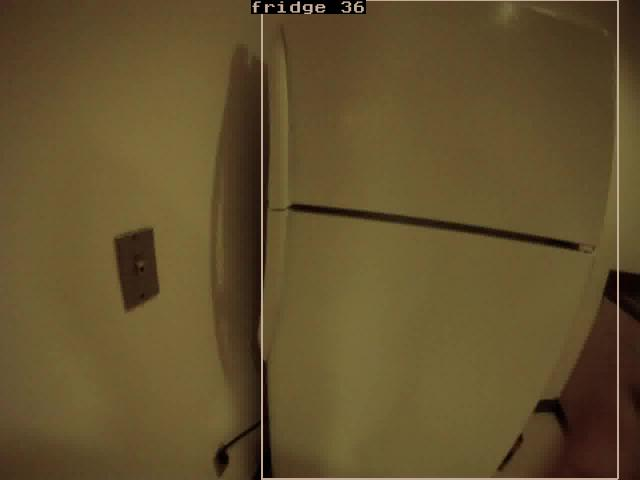
\includegraphics[width=3.0cm]{figures/fridge_passive.jpg}}}
\subfigure[passive soap]{\fbox{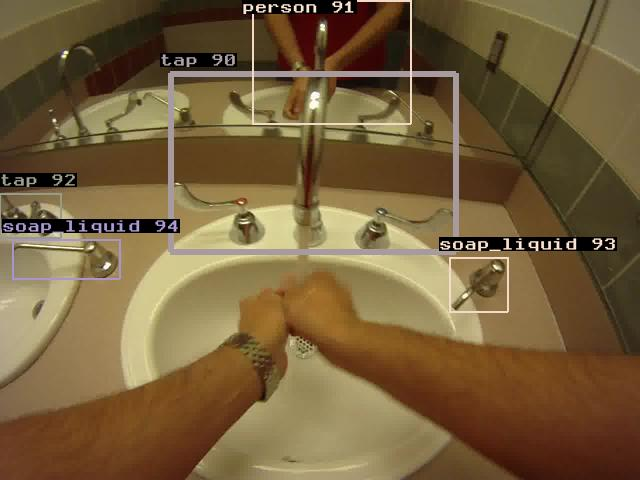
\includegraphics[width=3.0cm]{figures/soap_passive.jpg}}}
\subfigure[passive mug]{\fbox{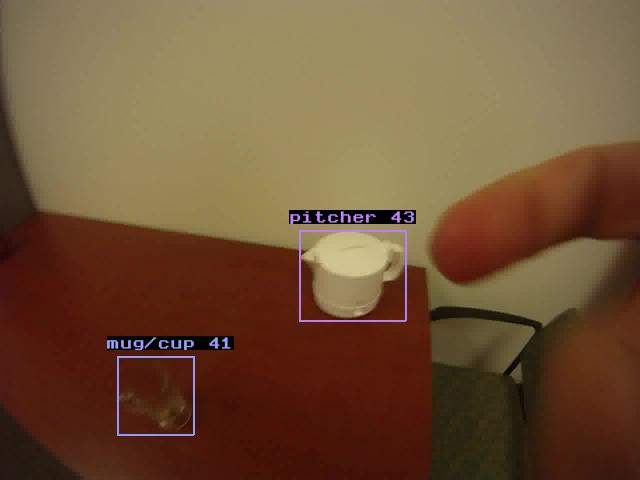
\includegraphics[width=3.0cm]{figures/mug_passive.jpg}}}
\subfigure[passive micro]{\fbox{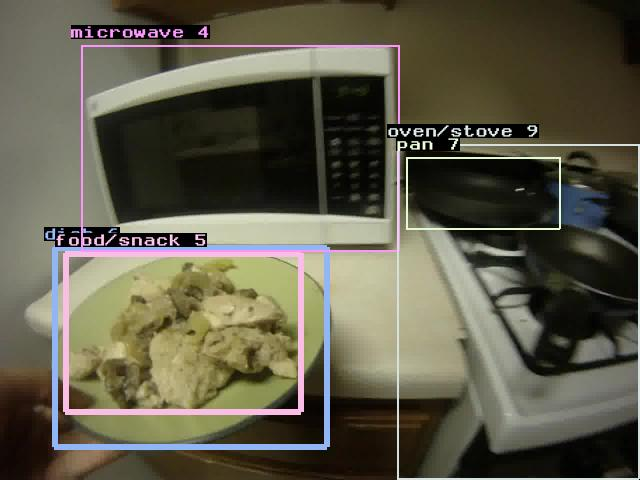
\includegraphics[width=3.0cm]{figures/micro_passive.jpg}}}\\
\subfigure[active frig]{\fbox{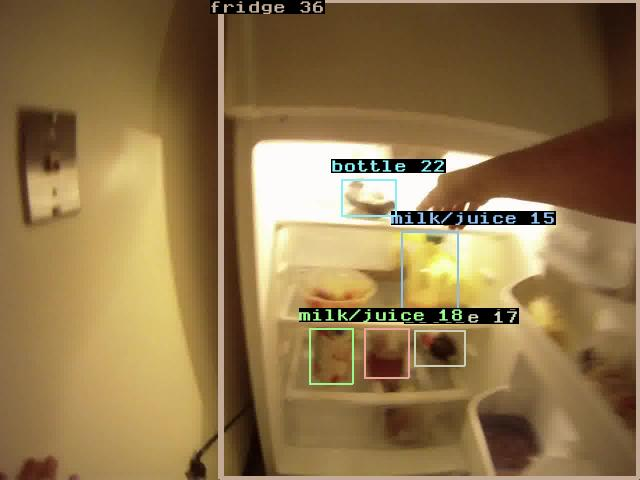
\includegraphics[width=3.0cm]{figures/fridge_active.jpg}}}
\subfigure[active soap]{\fbox{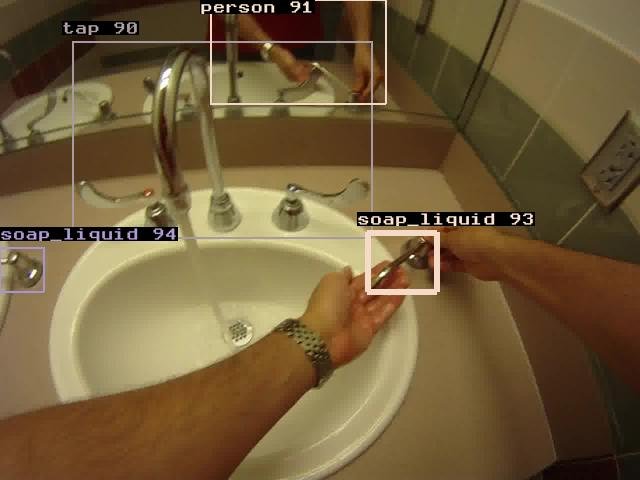
\includegraphics[width=3.0cm]{figures/soap_active.jpg}}}
\subfigure[active mug]{\fbox{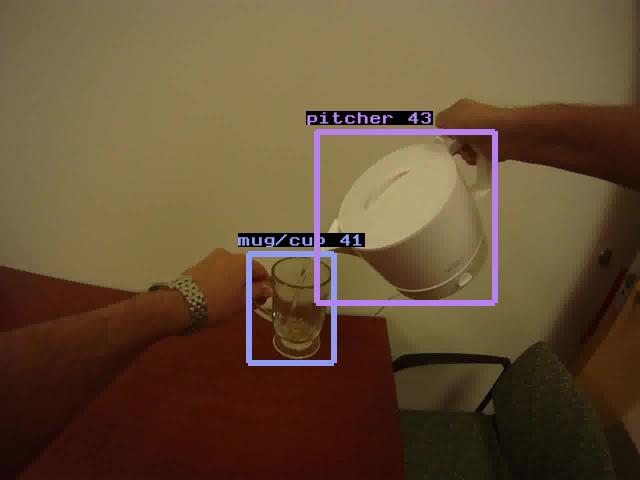
\includegraphics[width=3.0cm]{figures/mug_active.jpg}}}
\subfigure[active micro]{\fbox{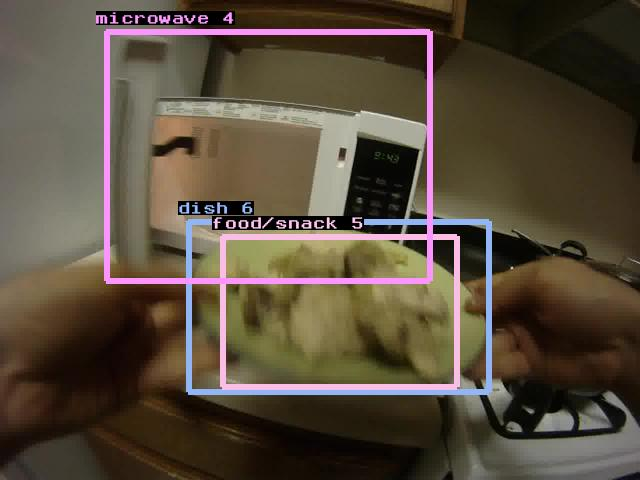
\includegraphics[width=3.0cm]{figures/micro_active.jpg}}}
\end{tabular}
		   \caption{Example passive and active instances of four objects in ADL \cite{Ramanan12}.}\vspace*{-0.2in}
\label{fig:active}
  \end{center}
 \end{figure}

  








  \subsection{Generating Randomized Object-Centric Space-Time Pyramids}

  Active objects, those which are being interacted with by the user in a
  given video clip, are especially helpful features for egocentric activity
  recognition \cite{Ramanan12}, yet there is little work in the literature
  exploring the best ways to pool video features across space-time. A common
  technique for pooling features is ``bag-of-words'', an orderless histogram
  of feature counts. This technique is simple, but does not encode any
  potentially useful relationships between features in space-time. The
  ``pyramid'' is an extension to bag-of-words that encodes space-time
  relationships between features by recursively
  subdividing an image or video into multiple subregions and concatenating
  bag-of-words histograms computed for each region. 

  Existing work relies on hand-coded partition schemes for computing
  pyramid representations of datapoints, which is a problematic approach
  because it is inflexible with respect to new data and can fail to capture
  the most meaningful relationships between features. To address this
  problem, we propose to randomly generate a pool of candidate partitioning
  schemes.

  A Randomized Spatio-Temporal Pyramid (RSTP)
  is generated using a hierarchical partitioning of feature space.
  We generate cuts independently in a round-robin manner over dimensions $(x, y, t)$. 
  Each cut is axis-aligned
  (we incorporate random shifts, but not random rotations).
  To construct a partition scheme that is easily applicable to videos of
  arbitrary size, we consider
  partitioning an ``idealized'' video clip that has all dimensions normalized
  to length 1. To generate a single cut we sample a random number from a
  uniform distribution subject to any constraints imposed by ``parent cuts'' and use
  this as a randomized offset for an appropriate axis-aligned plane. To
  construct an unbiased partition scheme we sample from a uniform
  distribution.
  
  To represent a video clip 
  using a particular partition scheme we use the output of object detectors
  trained in \cite{Ramanan12}, which gives bounding boxes and object
  labels for each extracted frame. We use centers of bounding boxes to
  obtain $(x,y,t)$ coordinates for each individual object.
  We compute histograms of detected
  objects for each individual level in the pyramid,
  where level 0 is the entire video clip volume and level $i$ is all the
  cells of depth $i$ in the pyramid. 
  Note that level $i$ has $8^i$ leaf
  cells. To form the final RSTP representation, we concatenate the
  histograms computed for each level to form a single feature vector.
  
  %now describe with bias
  There are many high-dimensional partition schemes that we could sample
  randomly, which suggests that a very large pool of candidate partition
  schemes is required to obtain good results. However, boosting is
  computationally expensive, so we would like to minimize the size of the
  pool while maintaining good results.
  One of the main contributions of our work is the ability to generate
  meaningfully biased randomized partition schemes that tend to be more discriminative
  than their unbiased counterparts.
  To accomplish this, we propose to replace the uniform distribution with a discrete
  approximation of the distribution of active objects across each dimension
  $(x, y, t)$
  and otherwise proceed normally.
 \begin{figure}
  \begin{center}
\begin{tabular}{ccc}
\fbox{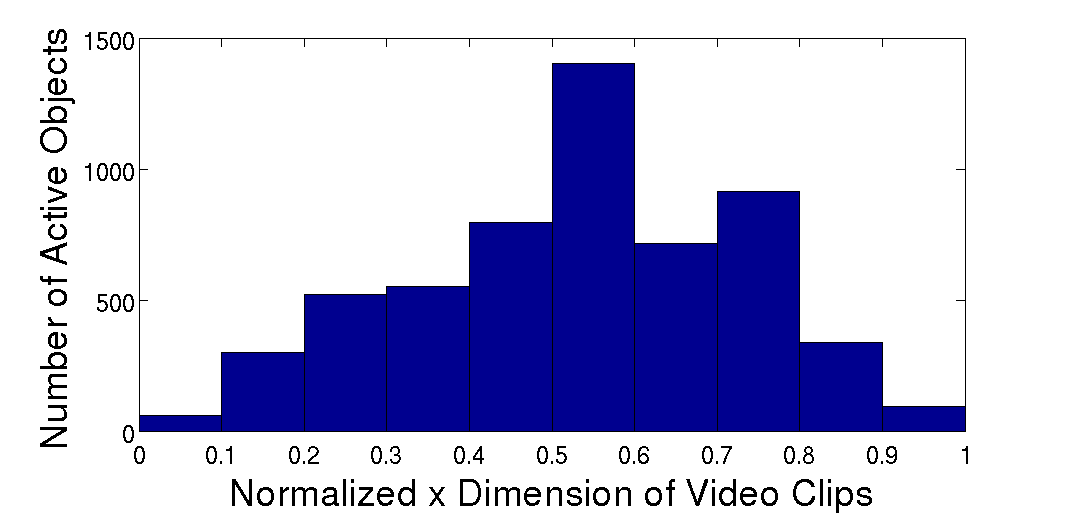
\includegraphics[width=4.4cm]{figures/active_obj_distr_x.png}}&
\fbox{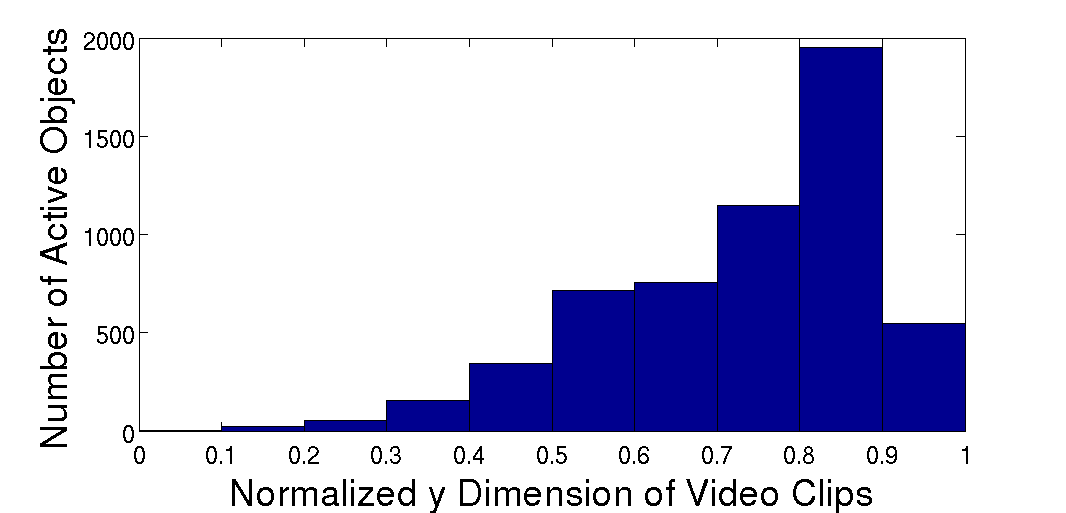
\includegraphics[width=4.4cm]{figures/active_obj_distr_y.png}}
\fbox{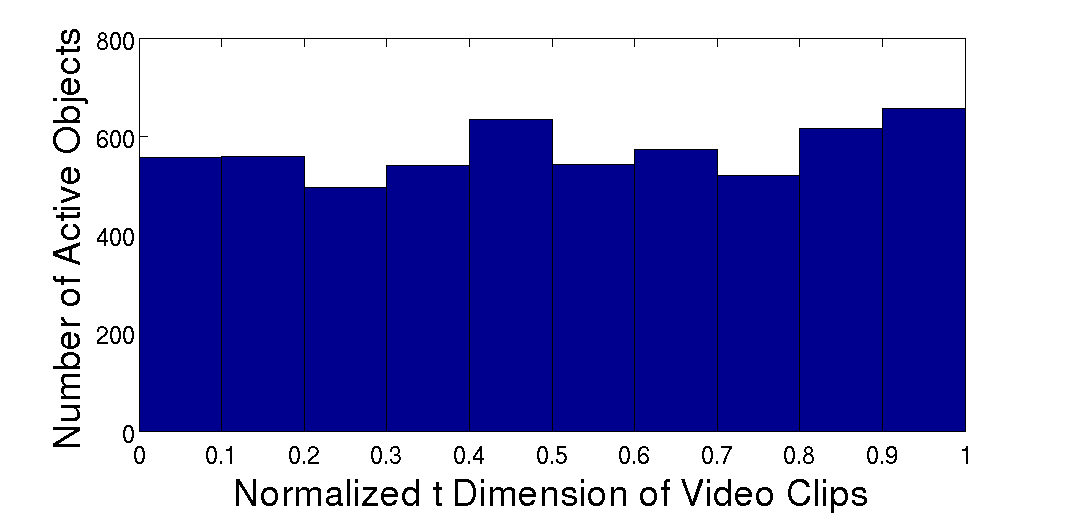
\includegraphics[width=4.4cm]{figures/active_obj_distr_t.png}}
\end{tabular}
		   \caption{Histograms of detected active objects across the $x$, 
       $y$, and $t$ dimensions of training data. }
\label{fig:histograms}
  \end{center}
\end{figure}
	 
  To generate Object-Centric Cuts (OCCs), we first compute histograms of active object
  locations across each $(x,y,t)$ dimension of the training data.
  Figure~\ref{fig:histograms} shows that active objects often tend to occur in the lower center
	of the field of view. This conforms to our expectations, because
	the active objects are close to the hands which are in the lower field of
	view from an egocentric perspective. Active objects tend to occur on the
  right side of the field of view slightly more often because a large
  percentage of users are right-handed.
  The distribution of active objects
  across the temporal dimension is nearly uniform. 
  This distribution is computed across all action types; we do not compute
  separate active object distributions for each action class.
  Since different clips can have
  varying lengths with respect to time, we normalize the length of each
  video clip to 1 and consider relative temporal locations of active
  objects. 
	For biased partitions, we generate
  the first split along each dimension according to a distribution
  corresponding to the histograms of observed active object coordinates in the training data,
  and we generate all subsequent child cuts using a uniform distribution.
  For example, when generating a biased cut for the $y$ dimension, 
  we generate a random number between 0 and 1 that has a high probability of
  being in the range $(0.5, 0.9)$.
  We do not consider locations of passive objects at all during the
  generation of biased partition schemes.
  Since active objects are located
  in close spatial proximity to hands, creating object-centric partition schemes can
  be interpreted as implicitly taking into account information about hand
  locations.



  Figure~\ref{fig:2dpartitions} depicts some example frames overlayed with
  randomized shifts sampled using our object-centric strategy (a) and the simple
  uniform strategy (b). The depicted object detections are from the ADL
  repository \cite{Ramanan12}. Object-centric cuts successfully focus the
  histogram bin boundaries on space-time regions where users interact with
  objects. Thus, they may offer useful discriminative cues to the boosted
  classifier.



\begin{figure}[t]
  \begin{center}
  \begin{tabular}{c}
  \subfigure[Object-centric cuts]{
\begin{tabular}{ccccc}
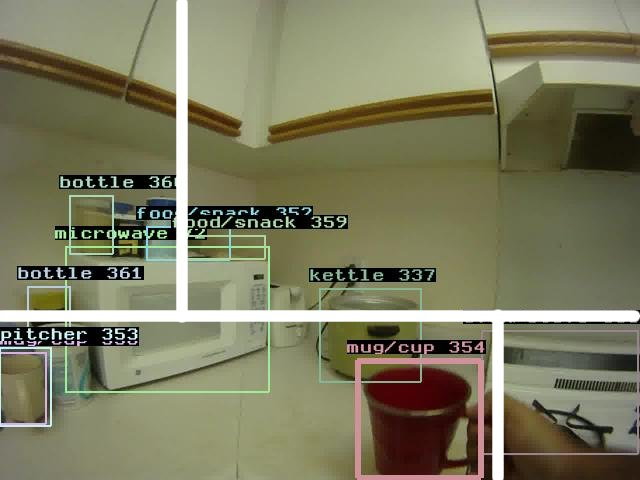
\includegraphics[width=2.2cm]{figures/ex1_biased.jpg}
%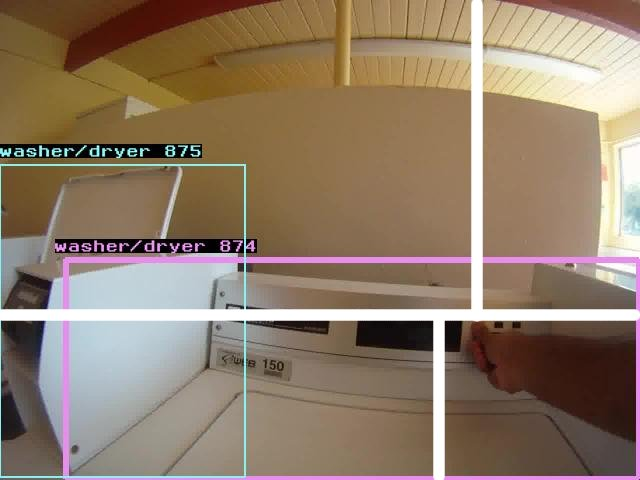
\includegraphics[width=2.2cm]{figures/ex2_biased.jpg}
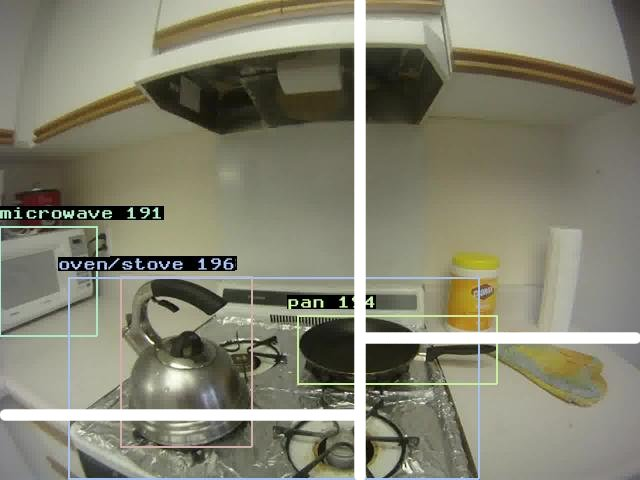
\includegraphics[width=2.2cm]{figures/ex3_biased.jpg}
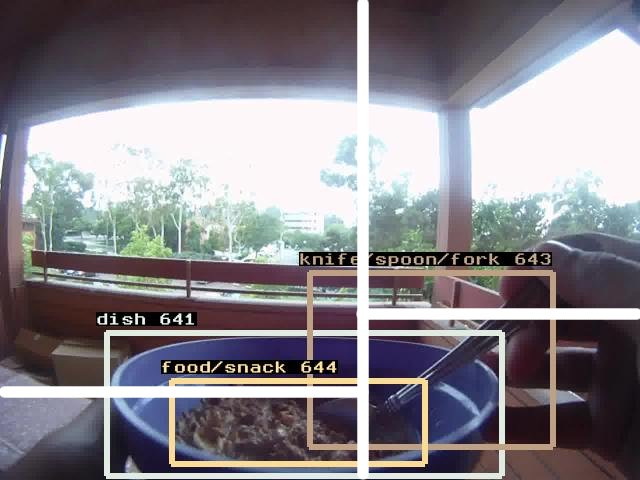
\includegraphics[width=2.2cm]{figures/ex4_biased.jpg}
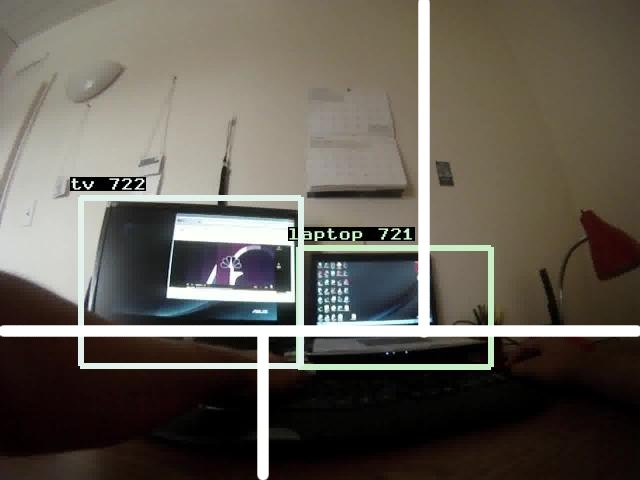
\includegraphics[width=2.2cm]{figures/ex5_biased.jpg}
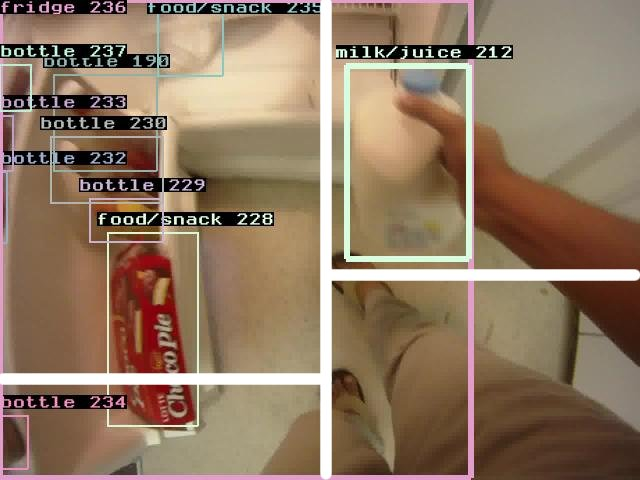
\includegraphics[width=2.2cm]{figures/ex6_biased.jpg}
\end{tabular}}\\
 \subfigure[Uniformly random shifts]{
\begin{tabular}{ccccc}
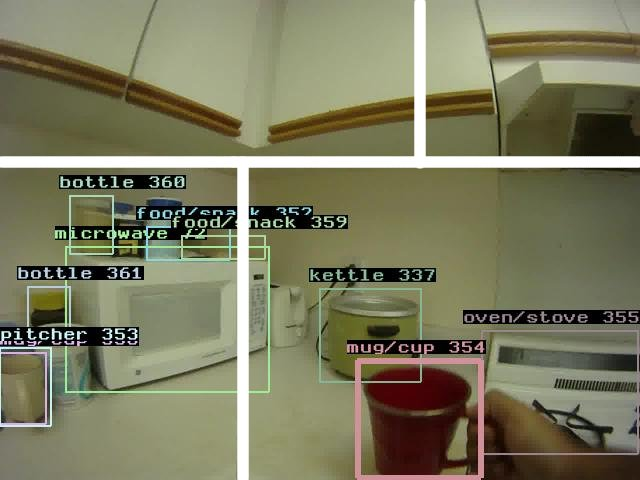
\includegraphics[width=2.2cm]{figures/ex1_unbiased.jpg}
%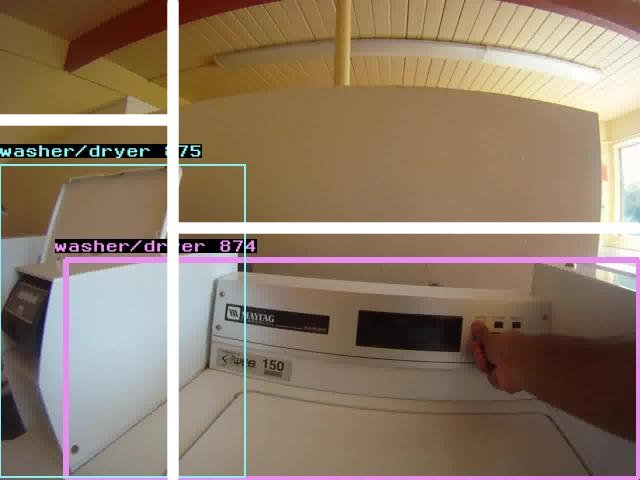
\includegraphics[width=2.2cm]{figures/ex2_unbiased.jpg}
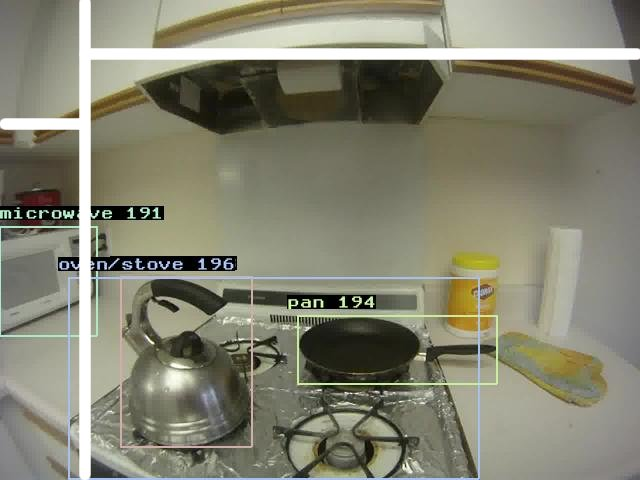
\includegraphics[width=2.2cm]{figures/ex3_unbiased.jpg}
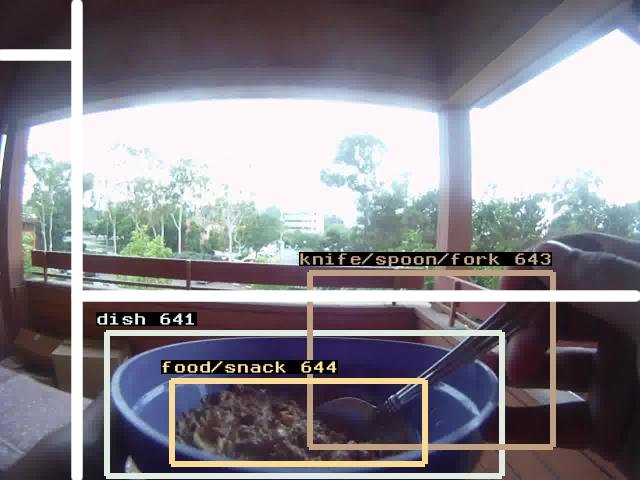
\includegraphics[width=2.2cm]{figures/ex4_unbiased.jpg}
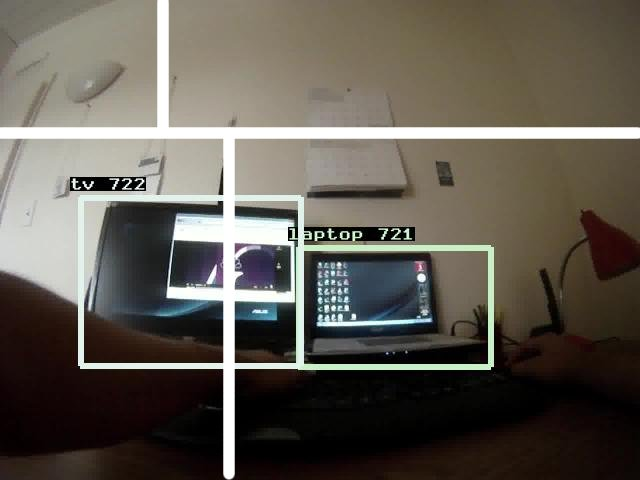
\includegraphics[width=2.2cm]{figures/ex5_unbiased.jpg}
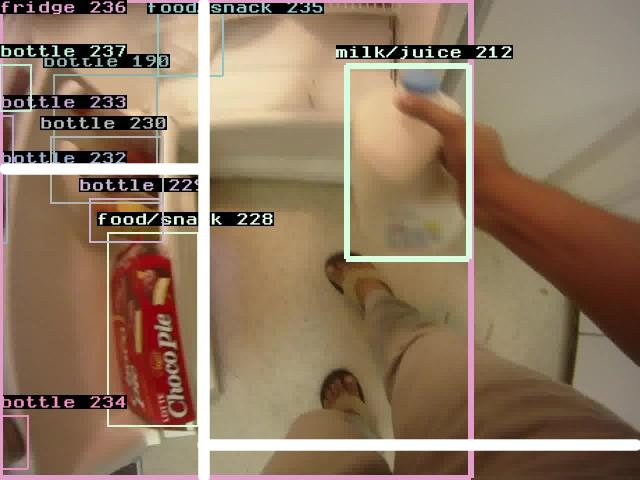
\includegraphics[width=2.2cm]{figures/ex6_unbiased.jpg}
\end{tabular}}
\end{tabular}
%\bmvaHangBox{\fbox{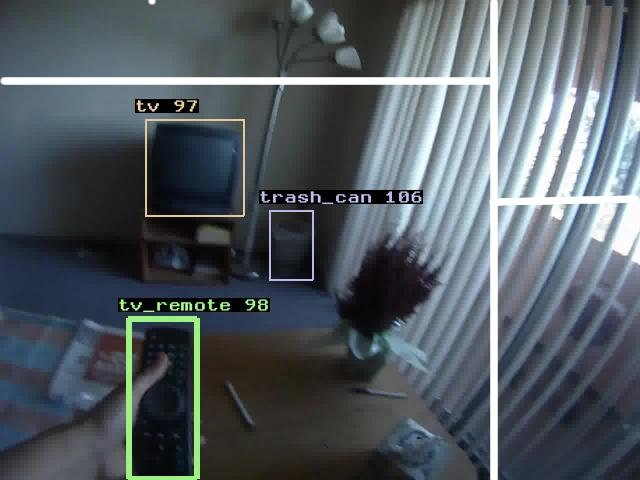
\includegraphics[width=5.9cm]{figures/unbiased_prt.jpg}}}&
%\bmvaHangBox{\fbox{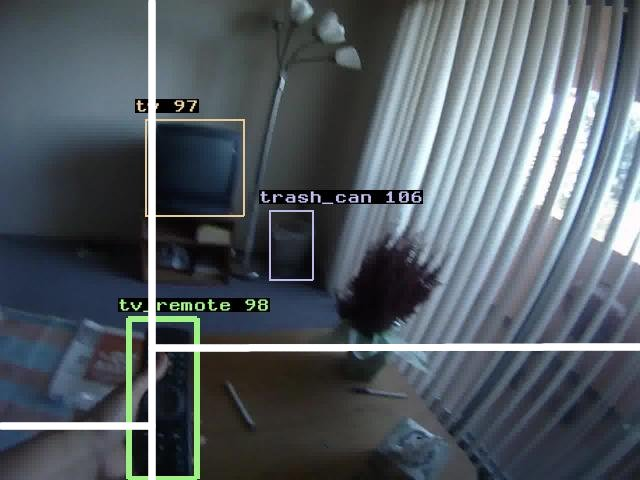
\includegraphics[width=5.9cm]{figures/biased_prt.jpg}}}\\
		   \caption{Example partitions using either object-centric (a) or uniformly sampled randomized cuts (b).  Note that for display purposes we show cuts on example 2D frames, but all cuts are 3D in space-time.  Using the proposed object-centric cuts, we better focus histograms surrounding the human-object interactions.}
\label{fig:2dpartitions}
  \end{center}
\end{figure}



	\begin{figure}[t]
		\begin{center}
			%\fbox{\rule{0pt}{2in} \rule{0.9\linewidth}{0pt}}
			  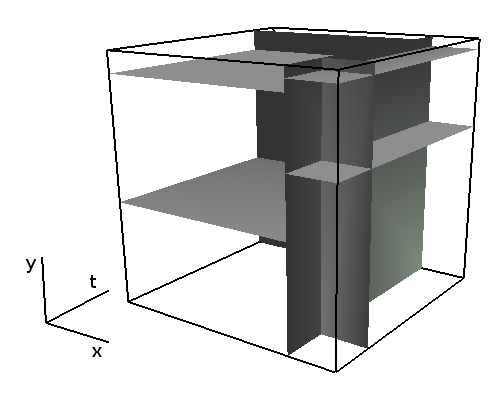
\includegraphics[width=6.0cm]{figures/biased.png}
		\end{center}
    \caption{An example 2-level object-centric partitioning scheme}
  
				\label{fig:3dpartition}
	\end{figure}
  
  Figure~\ref{fig:3dpartition} depicts an example 2-level object-centric partition scheme. 
  The salient feature to note is that visible splits along the $x$ and $y$
  dimensions correspond to the observed distribution of active objects along
  the $x$ and $y$ dimensions of the training data.
  






  \subsection{Boosting Discriminative Spatio-Temporal Pyramids}
  
\begin{figure}[t]
  \begin{center}
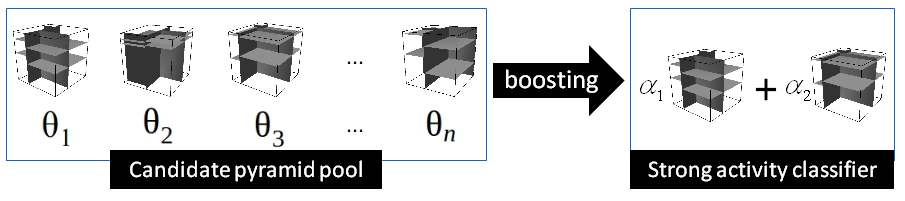
\includegraphics[width=13cm]{figures/concept-alg.png}
		   \caption{We take a pool of randomized space-time pyramids with object-centric cuts, and use boosting to select those that are most discriminative for egocentric activity recognition.}
\label{fig:concept-alg}
  \end{center}
\end{figure}


  Once we have constructed a pool of randomized object-centric pyramids, we use a
  boosting algorithm to select those which are most discriminative for egocentric
  activity recognition (see Figure~\ref{fig:concept-alg}).
 
  The intuition behind boosting is to train a set of ``weak'' classifiers (better
  than chance) and
  combine their output to form a ``strong'' classifier in such a way as to take advantage of the strengths
  of each individual weak classifier.
  This is accomplished by iteratively training classifiers on the training data.
  Datapoints are re-weighted after each iteration so that classifiers added during
  subsequent iterations tend to focus on examples that were previously
  misclassified. Each weak classifier is a non-linear (polynomial kernel) SVM
  trained using one RSTP with OCC's. 
  
  We use the Stage-wise Additive Modeling using a
  Multi-class Exponential loss function (SAMME) boosting approach of
  \cite{Zhu06}, which is a natural extension of the original AdaBoost algorithm
  to a multi-class classification task without a reduction to multiple binary
  classification problems. We selected this algorithm because it avoids training
  individual classifiers for multiple one-vs.-all or one-vs.-one classification
  problems.

	For our method, SAMME boosting works as follows. We take as input a collection of $N$ labeled training videos 
  where $(V_i, c_i)$ denotes a video clip and its associated ground-truth
  activity label,
	and a pool of $M$ candidate partition patterns 
  $\{\theta_1, \theta_2, ..., \theta_M\}$.
  We use the output of the
  aforementioned object detectors trained on composite object models as our features to be
  pooled. To convert from object bounding boxes to $(x,y,t)$ coordinates, we
  simply take the center of each bounding box.
  Thus, each training example $V_i$ is a set of $(o,x,y,t)$ object
  locations, where $o$ denotes an object label.

  To represent a particular training example $V_i$ using a particular
  partition scheme $\theta$, we compute separate bag-of-words histograms for
  each level in $\theta$, and concatenate all such histograms to form a
  final feature vector used in training.
  We initialize a weight
  $w_i$ for each
	training example $V_i$ that is inversely proportional to the number of points
	with the same class as $V_i$. Giving larger weights to training examples of
  infrequently occurring actions helps to mitigate any bias resulting from imbalanced
  training data.
  
  We train a separate ``weak''
  multi-class SVM 
  (using LIBSVM \cite{Chang11})
	classifier on the feature vectors resulting from representing the training
	data using each candidate partition pattern $\theta$.   During each round of boosting we select the
	candidate partition $\theta_j$ that is most discriminative (has minimum
  weighted training
	error, which is computed as the dot product between the weight vector $w$
  and an indicator of incorrect classifications using $f_\theta$).
  Next, we compute a weight for $\theta_j$ based on how many training
  examples were misclassified using $f_{\theta_j}$, the classifier
  that was trained using the representation of the training data under
  $\theta_j$.
  At the end of each boosting iteration, we update the weights for each
  training example. Training examples that were previously misclassified are
  assigned higher weights to encourage correct classification in future
  boosting rounds.
  Finally, we generate the 
	final strong classifier $F$, which maximizes a weighted
  sum of correct classifications produced by each weak classifier.

  Given a novel test video $V$, we compute object locations, then extract only those
  RSTP histograms that were selected during the boosting algorithm, and then
  apply $F$ to $V$ to robustly predict its activity label. Algorithm 1 summarizes
  these steps in more detail.\\
  
  \footnotesize
  \noindent\line(1,0){420}\\
  \textbf{Algorithm 1:} Training a space-time pyramid classifier with boosting \\
  \line(1,0){420}\\
  \textbf{\scriptsize INPUT:}
  \begin{itemize}
    \item $N$ labeled training videos $\Phi = \{(V_i, c_i)\}_{i=1}^N$
    \item A pool of $M$ partition patterns $\Theta = \{\theta\}$
  \end{itemize}
  \textbf{\scriptsize OUTPUT:}
  \begin{itemize}
    \item A strong video classifier $F$. For an unlabeled video $V$,
      $c=F(V)$ is the predicted label for $V$.
  \end{itemize}
      \begin{enumerate}
        \item For each pattern $\theta \in \Theta$:
          \begin{itemize}
            \item Represent each $V_i \in \Phi$ using $\theta$
            and train an SVM classifier $f_\theta$ on the
            resulting feature vectors.
          \end{itemize}

        \item Initialize:
          \begin{itemize}
            \item A weight vector $w$ with $w_i = \frac{1}{C N_{c_i}}$ for each video
              where
              $N_{c_i}$ is the number of videos with label $c_i$, and
              $C$ is the number of distinct action labels.
            \item Current boosting round $j=0$.
          \end{itemize}

        \item For each round of boosting:
          \begin{itemize}
            \item Increment $j$ and re-normalize the weight vector $w$.
            \item For each pattern $\theta$,
              compute its weighted classification error:
              $\;\;\;\;e_\theta = w \cdot \mbox{\textbf{I}}(f_\theta(V) \neq c)$
            \item Choose the pattern $\theta_j$ with minimum weighted
              classification error $e_j$.
            \item Compute the weight for $\theta_j$ as:
              $\;\;\;\;\alpha_j = \mbox{log} \frac{1 - e_j}{e_j} + \mbox{log}(C-1)$
            \item Update the weight vector $w$:
              $\;\;\;\;\forall i: w_i = w_i \cdot \mbox{exp}(\alpha_j \cdot
              \mbox{\textbf{I}}(f_{\theta_j}(V_i) \neq c_i))$.
            \item Generate the current strong classifier:
              $\;\;\;\;F(V) = \mbox{argmax}_c \Sigma_{m=1}^j \alpha_m \cdot
              \mbox{\textbf{I}}(f_{\theta_m}(V) = c)$
          \end{itemize}
      \end{enumerate}
  \line(1,0){420}\\
  \normalsize
  
  
	




  \subsection{Complexity and Training Time}
  The asymptotic complexity of training with $N$ training examples 
  and a pool of $M$ candidate partition schemes with $l$ levels using our
  method is 
  \begin{center}
  $O(N\cdot M \cdot 8^l \cdot t_{train} + b \cdot (N + M \cdot t_{test}))$
  \end{center}
  where $b$ denotes the number of boosting rounds, and $t_{train}$ and
  $t_{test}$ denote the time to train and test a single SVM classifier on
  $N$ feature vectors, respectively. Fortunately, $l$ remains small (never
  exceeds 4 in our experiments). In order to predict the label for a single
  test video clip $v$, we first need to compute representations of $v$ using
  each partition scheme that was selected during boosting, then find the
  class $c$ which maximizes a weighted sum of matching classifications using
  each weak classifier selected during boosting.
  Thus, the overall
  asymptotic complexity of predicting the
  label for a single video clip is 
  \begin{center}
  $O(b \cdot 8^l + C \cdot b \cdot t)$
  \end{center}
  where $b$ is the number of boosting rounds, $C$ is the number of possible
  activity labels, and $t$ is the time to predict the label of a test
  example using a weak SVM classifier.
  
\begin{figure}
  \begin{center}
\fbox{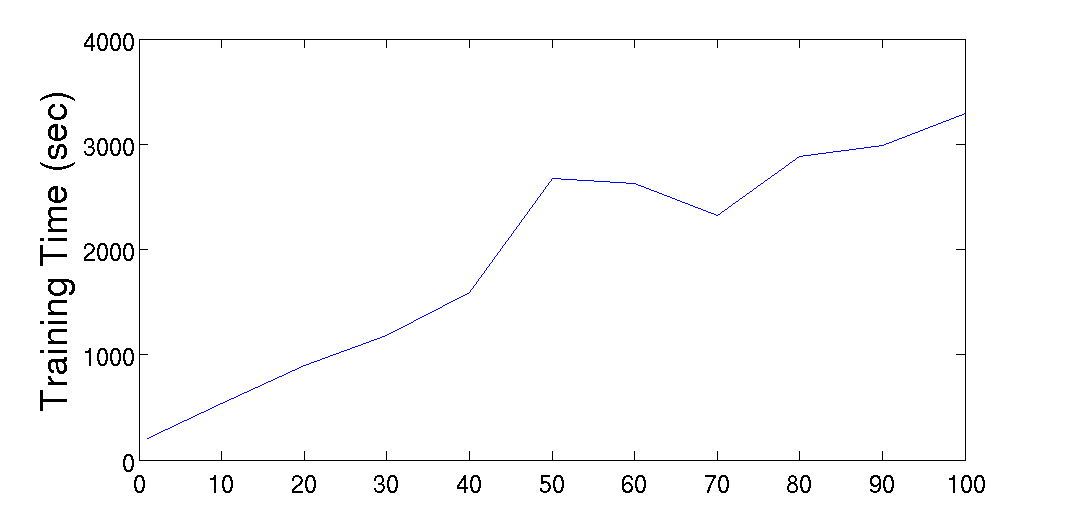
\includegraphics[width=9.0cm]{figures/runtime.png}}\\
		   \caption{Training times for our method as a function of pool size.}
\label{fig:runtime}
  \end{center}
\end{figure}
Figure~\ref{fig:runtime} depicts empirically determined training times for our method on a
  single ``fold'' of the cross-validation experiment described in section
  3.1. For each pool size we present mean execution time across 5 separate
  executions. Training time is linear with respect to pool size.
  

\section{Results}
  In this section we briefly describe properties of the dataset we use to
  benchmark our method and present results from experiments we conducted. We
  evaluate our overall recognition accuracy and show that it improves the
  current state of the art, and we demonstrate the superior discriminative
  power of object-centric partition schemes.

  The ADL dataset consists of hundreds of egocentric video clips
	(roughly 10 hours of video in total) collected from 20 people performing
	18 types of unscripted actions in their own homes. These naturally
  occurring
  actions are often related to hygiene or food preparation and are more
  varied than actions presented in previous datasets such as that of \cite{Fathi11}.
  There are 26 different 
	types of detected objects, including 5 active and 21 passive objects. 
  Lists of activity types and object types are given in Table~\ref{table:adl}.
  Object detectors are trained on videos from the
  first 6 people and tested on the videos from the remaining 14 people.

  
\begin{table}
  \begin{center}
\begin{tabular}{cc}
\fbox{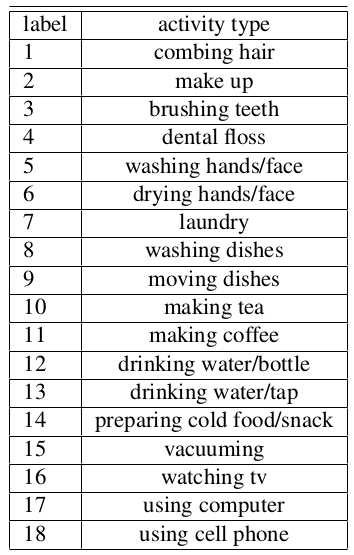
\includegraphics[width=4.0cm]{figures/actionlist.png}}&
\fbox{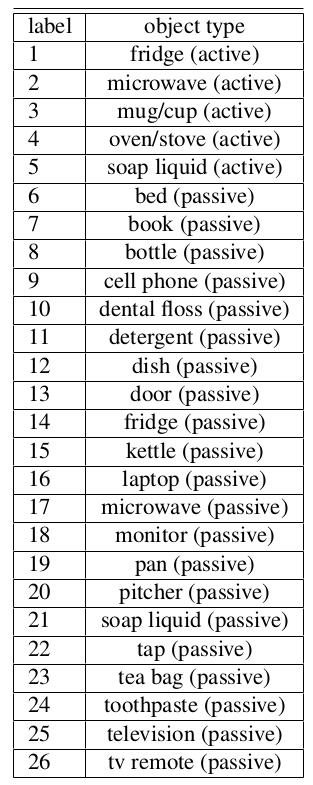
\includegraphics[width=4.0cm]{figures/objectlist.png}}\\
\end{tabular}
		   \caption{Lists of action types and object types present in the
       ADL dataset. Separate active and passive models are trained for fridge,
     microwave, mug/cup, oven/stove, and soap liquid.}
\label{table:adl}
  \end{center}
 \end{table}
  

  
	Each frame in the dataset
	is annotated with activity labels and bounding boxes for automatically detected objects and hand positions, 
	Additionally, each object is tagged as active or passive depending
	on whether it is being interacted with. 
  
  One difficulty that can arise within egocentric
  activity recognition is that activities can be temporarily interrupted by
  other activities. For instance, while waiting for tea to brew a subject
  may watch TV. For cases of such interruptions, to avoid unnecessary
  complications resulting from frames being annotated with multiple
  activities, the ADL dataset simply uses the label of the interrupting
  action when a longer action is disrupted.
  

	The ADL dataset has been modified since the publication of
	\cite{Ramanan12}; because of this, running the published code gives
	slightly lower accuracy than the originally published numbers. We use the
  modified version of the dataset available from the authors webpage at the time of writing to
  benchmark our method.   \subsection{Action Recognition Performance}
  Following \cite{Ramanan12}, we evaluate recognition performance on the ADL
  dataset using a form of cross
	validation (the video clips from person $i$ are used as a held out validation set, and
	training occurs using the video clips from the remaining people).
  We exclude videos from the first 6 people
  (because they were used to train the object detectors) from our
  experiments.

	For this experiment we tried pools of 4-level partitioning schemes of
  varying sizes with a varying number of boosting rounds. We used 5 boosting rounds and a pool of
  size 70.
  These results were obtained
  using both active (being interacted with) and passive detected objects.
  
  Table~\ref{table:results} shows a comparison of overall classification accuracy between our
  approach and the method based on temporal pyramids which is
  presented in \cite{Ramanan12}. The first baseline, bag-of-words uses space-time
  interest points, a standard representation for action recognition in the
  third-person case. The second baseline uses a bag of detected objects. The
  third baseline, the temporal pyramid as first proposed in \cite{Ramanan12},
  has two levels, formed by making a single cut along the temporal
  dimension and no cuts along the spatial dimensions. The temporal pyramid
  represents the state of the art on this dataset. The fourth baseline, RSTP, is
  similar to our proposed approach, except it uses cuts sampled from a uniform
  distribution instead of object-centric cuts.
  
  Our approach outperforms all four baselines, improving on the state of the art.
  Compared to the bag of words approach, our method has the advantage of using
  high-level features (object coordinates). The temporal pyramid also has this
  advantage, but relies on a manually defined binning structure, making it
  weaker than our proposed method. Object-centric cuts are essential for our
  recognition result, as simply using cuts drawn from a uniform distribution
  leads to noticeably weaker performance. This supports our claim that biasing
  bins according to human-object interactions provides useful cues for
  recognition in an egocentric context.

    \begin{table}
		\begin{center}
			\begin{tabular}{|l|c|c|c|c|c|}
				\hline
        BoW & Bag-of-objects & TempPyr~\cite{Ramanan12} & Boost-RSTP & Boost-RSTP+OCC (ours) \\
				\hline\hline
        16.5\% & 34.9\% & 36.9\% & 33.7\% & \textbf{38.7\%}\\
				\hline
			\end{tabular}
		\end{center}
		\caption{Overall classification accuracy on ADL. Our method improves the state of the art.}\label{table:results}
	\end{table}




  
  \begin{figure}
  \begin{center}
  \begin{tabular}{cc}
  \subfigure{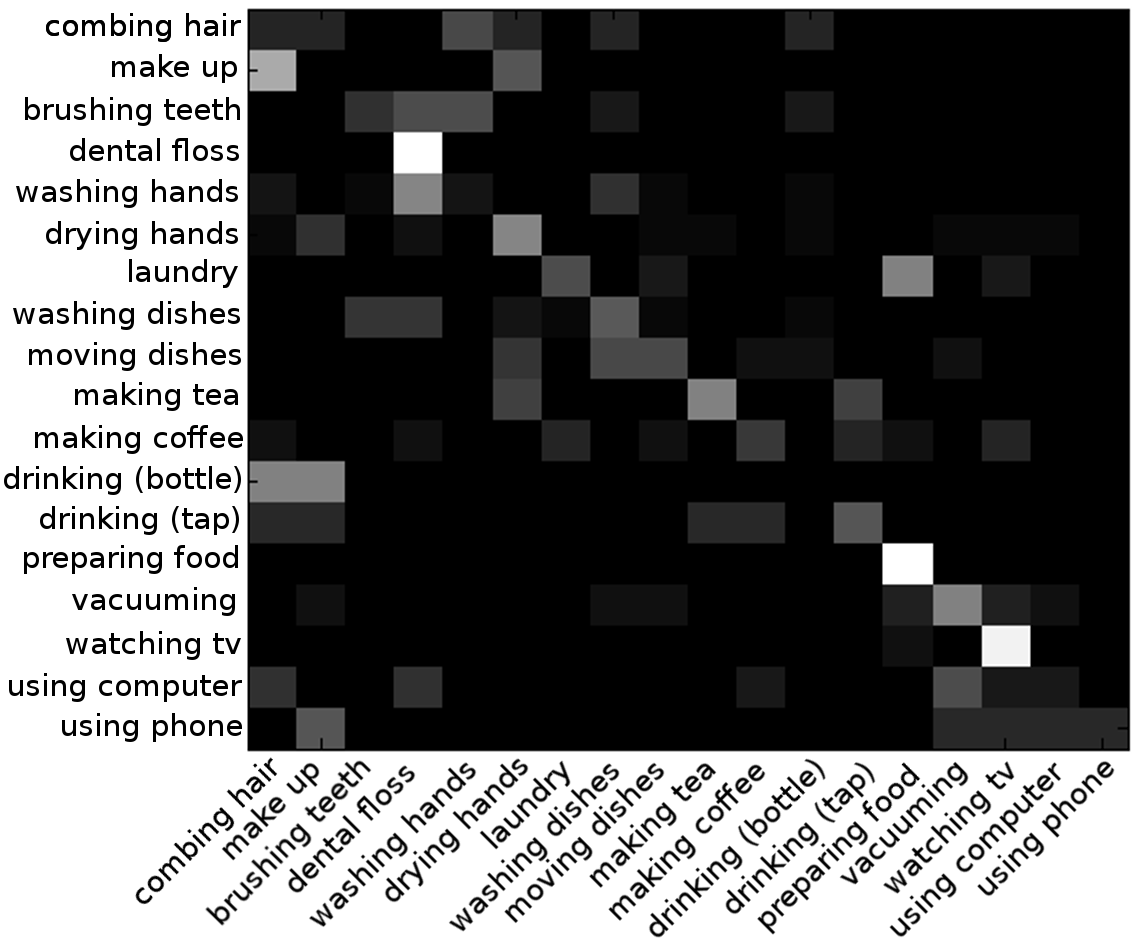
\includegraphics[width=7.0cm]{figures/ramananconfn.png}}
  \subfigure{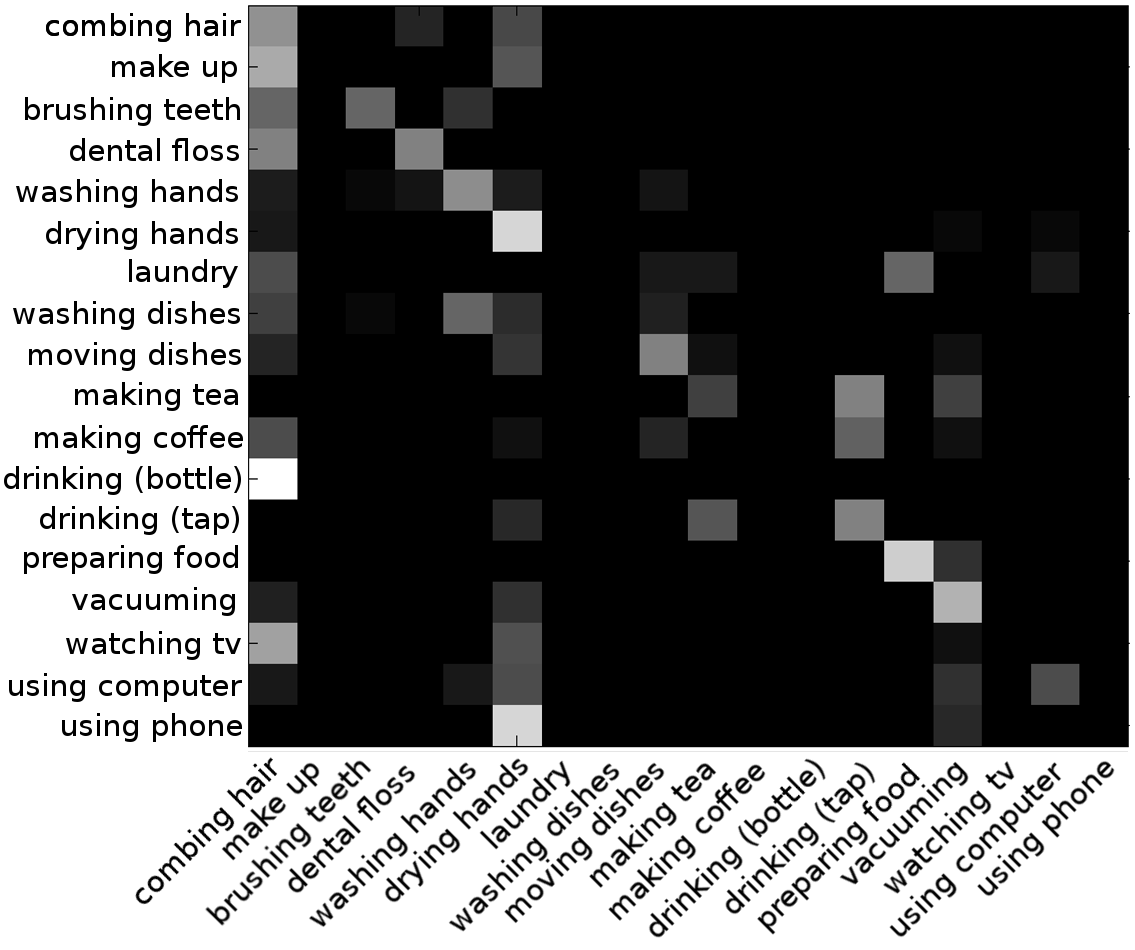
\includegraphics[width=7.0cm]{figures/ourconfn.png}}
  \end{tabular}
  \caption{Confusion matrices for temporal pyramid \cite{Ramanan12} (left, 36.9\%)
  and RSTP+OCC using detected active and passive objects (right, 38.7\%).}
  \label{fig:confn}
  \end{center}
  \end{figure}
  As seen in Figure~\ref{fig:confn}, our method has particularly good
  performance for ``combing hair'' and ``drying
  hands/face'', suggesting that our boosting approach was able to usefully
  isolate the space-time relationships present in these actions.
  The temporal pyramid likely yields worse performance on ``combing hair'' and ``drying
  hands/face'' because a single cut along the temporal dimension is not
  sufficient to isolate the relevant space-time relationships.
  This indicates that the spatial cuts we learn are essential for scenes with
  similar objects throughout different action. For example, floss or toothpaste
  might be visible on the counter while the user is combing hair, but when
  actually in use, floss or toothpaste would appear higher in the field of view.
  
  On the other hand, some action types on which we do
  poorly are ``making tea'' and ``making coffee''
  respectively (see Table \ref{table:adl} for a full listing of activity types present in
  the ADL dataset). Since the two activity types are similar in the sense that
  they involve the same active objects, it is not
  unexpected that a recognition system would confuse them often.
  Furthermore, since the distributions of objects across space-time are
  similar, and kettles and tea bags are not modeled in an active way, it is
  difficult for our boosting algorithm to select partitioning schemes that
  are discriminative for these classes. An extension of our method which
  allowed selection of discriminative partition schemes on a per-class basis
  could allow for more fine-grained control and could help mitigate such
  issues, however this is left for future work.




  

  % training error exp
  \subsection{Effect of Object-Centric Partition Schemes}
  To concretely illustrate the improvement obtained from using a
  object-centric partitions, we created separate pools containing 4-level
  partition schemes of each bias type and
  repeatedly ran our boosting algorithm, computing training error and adding additional
  partitions to each pool between runs. Results from this experiment are
  depicted in Figure~\ref{fig:trainerror}. The pool containing object-centric partitions 
  usually had a lower training error than the unbiased pool.
  Larger improvements are visible with smaller pool sizes, and the difference
  between the two pools diminishes as pool size increases. This conforms to
  expectations because as the unbiased pool grows in size, it becomes more
  likely to contain discriminative partition schemes, while the biased pool
  is forced to contain discriminative partition schemes even at relatively
  small pool sizes. This result suggests that by using object-centric
  partitions rather than unbiased partitions, we can obtain good recognition
  results even with a smaller pool, making our boosting algorithm less expensive
  to compute.
 
  \begin{figure}[t]
		\begin{center}
			%\fbox{\rule{0pt}{2in} \rule{0.9\linewidth}{0pt}}
			  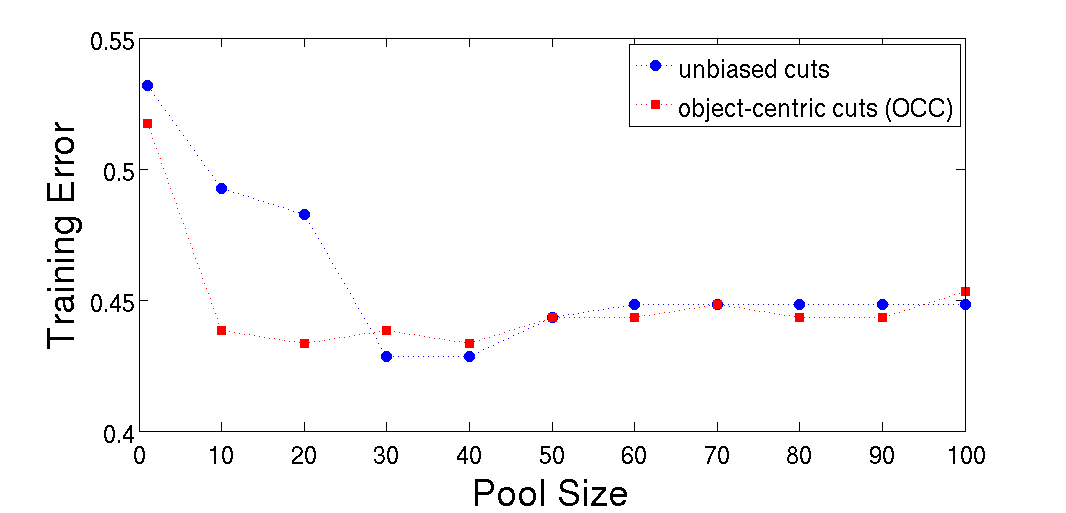
\includegraphics[width=10cm]{figures/trainerror.png}
		\end{center}
		   \caption{Effect of using biased partition schemes. The object-centric
         pool
       usually has lower training error
       than the pool of unbiased partition schemes. The most significant
     improvement is visible at smaller pool sizes.}
				\label{fig:trainerror}
	\end{figure}
  
	
\section{Conclusion and Future Work}
	Our main novel contribution is two-fold. We show how to learn the most
  discriminative partition schemes for spatio-temporal binning in video feature space, and
  we introduce object-centric partition schemes, which have a high
  probability of cutting through video regions known to frequently contain
  active objects. Unlike previous work, we randomly generate a pool of
  candidate partitioning schemes and select those which are most
  discriminative using a boosting algorithm.
  Our recognition approach improves on the current state of the art, and our
  experiments demonstrate the positive impact of taking active object
  locations into account by generating object-centric partition schemes.
  
  In future work, we intend to investigate ways of learning the most
  discriminative partition schemes on a per-class basis.
	Additionally, it may be possible to incorporate different types of biases when generating
	partitions. The ADL dataset also includes annotations for hand positions,
	which we have incorporated implicitly through our generation of
  object-centric cuts.
	However,
	it could be possible to incorporate explicit information given by hand
	positions to obtain better results.
	The partitions we focus on contain cuts that are
  planar and axis-aligned (we consider random shifts but not random
  rotations, and we do not consider non-planar splits),
  but it is possible to carve up the
	video volume in more advanced non-linear ways. Such a method would 
  make histogram computation more expensive, but may yield a more discriminative
	partitioning scheme that could lead to better classification accuracy.


%----------------------------------------------------------------------------------------
%	BIBLIOGRAPHY
%----------------------------------------------------------------------------------------
\bibliographystyle{bmvc2k}
\bibliography{egbib}

%----------------------------------------------------------------------------------------

\end{document}
